\begin{figure}
\begin{fullpage}
        \begin{center}
        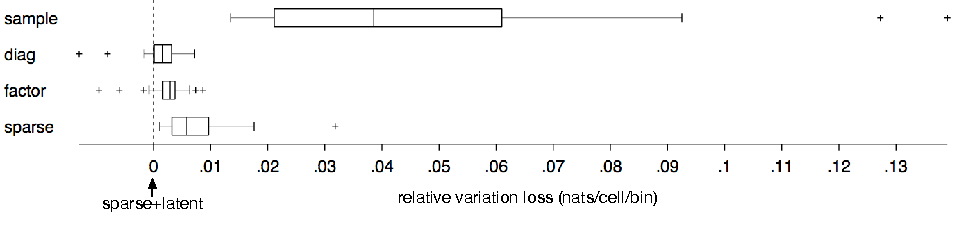
\includegraphics[width=\textwidth]{./figures/Figure4.pdf}
        \end{center}
\caption[Evaluation of correlation estimators by cross-validation]
{{\bf Evaluation of correlation estimators by cross-validation} 
The plot depicts the the validation losses (eq.~\ref{eq:vloss}) of estimators $C_{\sf sample}$, $C_{\sf diag}$, $C_{\sf factor}$, and $C_{\sf sparse}$ minus the validation loss of $C_{\sf sparse+latent}$ indicated by the dashed vertical line.
The difference is consistently positive ($p<0.01$ in each comparison, Wilcoxon signed rank test, $n=27$ sites in 14 mice), indicating that $C_{\sf sparse+latent}$  consistently outperforms the other estimators in these neural data.
The box plots indicate the $25^{th}$, $50^{th}$, and $75^{th}$ percentiles with the whiskers extending to the minimum and maximum values after excluding the outliers marked with `+'.
}\label{fig:4}
\end{fullpage}
\end{figure}
